% ch/maxwald2.tex: sections of Chapter chap:maxwald, the material of lines 349 to 569 of the manuscript (editor E2). Every number marked CHECK maxwald is replaced by the value of code/maxwald_*.py (data/maxwald_*.json).

\section{Is the clock a weak limit of GGC laws?}\label{mw:sec:weak}

The class of GGC laws is closed under weak limits \cite[Theorem 3.1.5]{Bondesson} (Section~\ref{sec:weak:limits}), and with Proposition~\ref{prop:rigid} this gives a sharp answer: $T$ is a weak limit of GGC laws if and only if RH holds (Corollary~\ref{cor:weak:closure}).

The de Bruijn Newman flow of Section~\ref{ch:dbn} is the second family of candidates, and Theorem~\ref{rz:thm:dbn} places RH at the end of a path of GGC laws. Let $\Phi_{\mathrm{dBN}}(u)=\frac12\Phi(2u)$ be the kernel in the rescaled variable of Rodgers and Tao \cite{RodgersTao}, as in Theorem~\ref{rz:thm:dbn}, let $H_t(z)=\int_0^\infty e^{tu^2}\Phi_{\mathrm{dBN}}(u)\cos(zu)\,du$ be the de Bruijn Newman deformation of $H_0(z)=\frac18\xi(\frac12+\frac{iz}2)$, with $\Lambda$ the de Bruijn Newman constant in this normalisation, and let $V_t$ be the variable with density proportional to $e^{tu^2}\Phi_{\mathrm{dBN}}(u)$, the Gaussian tilt of the P\'olya variable $V_0=X/2$, so that $\E e^{sV_t}=H_t(is)/H_t(0)$ for real $s$. Whenever a law $T_t$ makes $(T_t,V_t)$ a Wald couple (Definition~\ref{mw:def:wald}), $\E e^{-\lambda T_t}=H_t(0)/H_t(i\sqrt{2\lambda})=R_t(\lambda/2)$, where $R_t(u)=H_t(0)/H_t(2i\sqrt u)$ is the transform of the flow clock of Section~\ref{ch:dbn} and $R_0=1/G$. Thus $T_t$ is half the flow clock, and $T_0=T/2$; at $t=0$ the couple $(T/2,X/2)$ is the one of Remark~\ref{mw:rem:waldT} rescaled by $\sqrt2$.

By Theorem~\ref{rz:thm:dbn}, for every $t\ge\Lambda$ the transform $R_t$ is that of a GGC with Thorin measure $\sum_k\delta_{(z_k(t)/2)^2}$, where $z_k(t)>0$ are the positive zeros of the even function $H_t$ (each pair $\pm z$ gives one atom). Hence for $t\ge\Lambda$ the law $T_t$ exists and is a GGC with Thorin measure $\sum_k\delta_{z_k(t)^2/2}$, and since $\Lambda\le0.2$ \cite{PT21,Polymath} this holds unconditionally for $t\ge0.2$. As $t\downarrow0$, $H_t\to H_0$ locally uniformly, so $R_t(\lambda/2)\to1/G(\lambda/2)$ pointwise, which is the transform of $T/2$, and $T_t\to T/2$ in law along any sequence $t_n\downarrow0$ for which $T_{t_n}$ exists. With the bound $\Lambda\ge0$ of Rodgers and Tao \cite{RodgersTao}, Theorem~\ref{rz:thm:dbn} gives that RH holds if and only if $T_t$ is a GGC for every $t>0$, if and only if $\Lambda=0$.

Two cautions. Unconditionally $T_t$ is known to exist only for $t\ge0.2$ and at $t=0$ (Theorem~\ref{thm:ch12:idsd}), so the convergence $T_t\to T/2$ is a statement about the range of $t$ on which $T_t$ exists. Under RH this is every $t\ge0$; without RH, whether $T_t$ exists as a probability law for $0<t<0.2$ is open (Problem~\ref{mw:prob:flow} in Section~\ref{mw:sec:open}). And the Thorin atoms $z_k(t)^2/2$ of $T_t$ move with the zeros of $H_t$ only on the range $t\ge\Lambda$ where $T_t$ is a GGC; Table~\ref{tab:ch21:flowzeros} gives the zeros of $H_t(2\theta)$, in the variable $\theta=z/2$.

\begin{definition}[Laplace distance]\label{mw:def:laplace}
For laws $P$ and $Q$ on $[0,\infty)$ with Laplace transforms $L_P$ and $L_Q$, the Laplace distance is $d_L(P,Q)=\sup_{\lambda\ge0}|L_P(\lambda)-L_Q(\lambda)|$.
\end{definition}

\begin{proposition}\label{mw:prop:approx}
Let $H=3\times10^{12}$, let $N=N(H)$ be the number of zeros $\rho_k$ with $0<\gamma_k\le H$, and let $T^{[N]}=\sum_{k\le N}e_k/\gamma_k^2$ with independent standard exponential variables $e_k$, the GGC with transform $1/G_N$ of Section~\ref{sec:weak:limits}. With $a_k$ as in Section~\ref{ch:clock}, put $\varepsilon_H=\sum_{k>N}1/|a_k|$ and, for $K\le N$, $S_K=\sup_{\lambda\ge0}\lambda/G_K(\lambda)$. Then
\begin{equation}\label{mw:eq:approxbound}
d_L\big(T,T^{[N]}\big)\le S_K\,\varepsilon_H,\qquad \varepsilon_H<1.4798\times10^{-12},\qquad S_1=\gamma_1^2,\qquad S_{1700}<16.85,
\end{equation}
so that $d_L(T,T^{[N]})<2.5\times10^{-11}$, while the first factor alone gives $\gamma_1^2\varepsilon_H<2.96\times10^{-10}$.
The proof uses only the verification of RH up to height $H$ \cite{PT21}, and makes no assumption on the zeros above $H$.
\end{proposition}

\begin{proof}
By \eqref{eq:ch2:hadamard}, $1/G=\prod_kf_k$ with $f_k(\lambda)=(1+\lambda/a_k)^{-1}$, and $\re a_k=\gamma_k^2-(\beta_k-\frac12)^2>0$ for every zero, so for $\lambda\ge0$ we have $|1+\lambda/a_k|\ge\re(1+\lambda/a_k)\ge1$, hence $|f_k|\le1$ and $|f_k-1|=|\lambda/a_k|\,|f_k|\le\lambda/|a_k|$. For complex numbers of modulus at most one, $|\prod_jf_j-1|\le\sum_j|f_j-1|$. The zeros with $k\le N$ lie on the line, so $\prod_{k\le N}f_k=1/G_N$ is the transform of $T^{[N]}$, and its factors lie in $(0,1]$; leaving out all but the first $K$ of them can only increase the product, so $1/G_N\le1/G_K$. Therefore
\[
\Big|\frac1{G(\lambda)}-\frac1{G_N(\lambda)}\Big|=\frac1{G_N(\lambda)}\,\Big|\prod_{k>N}f_k(\lambda)-1\Big|\le\frac{\lambda}{G_K(\lambda)}\,\varepsilon_H\le S_K\,\varepsilon_H.
\]
For $K=1$, $\lambda/G_1(\lambda)=\lambda/(1+\lambda/\gamma_1^2)$ increases to $\gamma_1^2$, a supremum that is not attained. For $K\ge2$, $\frac d{d\lambda}\log(\lambda/G_K(\lambda))=-\phi_K(\lambda)/\lambda$ with $\phi_K(\lambda)=\sum_{k\le K}\lambda/(\lambda+\gamma_k^2)-1$, which increases strictly from $-1$ to $K-1$, so $\lambda/G_K$ increases up to the root $\lambda^*$ of $\phi_K$ and decreases after it. For $K=1700$ the root is $\lambda^*=47.362$, and evaluating $\phi_{1700}$ and $\lambda/G_{1700}$ in ball arithmetic with the first $1700$ zeros, on both sides of $\lambda^*$, gives $S_{1700}<16.8497$ (code/maxwald\_weak.py).

For $\varepsilon_H$, $|a_k|=|\rho_k-\frac12|^2\ge\gamma_k^2$, and partial summation gives $\varepsilon_H\le\sum_{\gamma_k>H}\gamma_k^{-2}=2\int_H^\infty(N(t)-N(H))\,t^{-3}\,dt$. Write $N(t)=N_0(t)+E(t)$ with $N_0(t)=\frac t{2\pi}\log\frac t{2\pi e}$; by \cite[Corollary~1.2]{HSW22}, $|E(t)|\le0.1038\log t+0.2573\log\log t+9.3675$ for $t\ge e$. The main term integrates to exactly $(\log\frac H{2\pi}+1)/(2\pi H)=1.47970\times10^{-12}$, and the bound for $E$, used at $t$ and at $H$, adds less than $10^{-23}$.
\end{proof}

\section{The sine squared lemma and the basepoint family in the \texorpdfstring{$\lambda$}{lambda} chart}\label{mw:sec:basepoint}

The sine squared lemma \eqref{eq:sin2} \cite[Lemma 8.1]{P17} turns the L\'evy measure of $\log\xi$ at a basepoint $\alpha$ into the Thorin measure of the reciprocal at the same basepoint. For $\alpha>1$ its input is the signed canonical measure of \cite[Theorem 8.1]{P26}; for $\frac12<\alpha\le1$ there is no such L\'evy form, and the family is defined by the Hadamard product, not by the lemma. The family is that of the shifted clocks $T_\alpha$ with transform $\varphi_\alpha(\lambda)=\xi(\alpha)/\xi(\alpha+\sqrt\lambda)$, $T_{1/2}=T$. For every $\alpha>\frac12$ put $u_\alpha(\lambda)=\re(\xi'/\xi)(\alpha+i\sqrt\lambda)/(2\pi\sqrt\lambda)$, the Thorin density of $T_\alpha$ when every zero has $\beta<\alpha$ (Theorem~\ref{thm:poisson}) and in every case the density of $U_\alpha$ of \eqref{eq:Ualpha} in the chart $\lambda=\theta^2$, a sum over the zeros of Poisson kernels (Proposition~\ref{prop:struct}), and for $\alpha>1$ it has the arithmetic form \eqref{eq:split} with $\theta=\sqrt\lambda$ (drift, archimedean, pole and prime pieces), which Table~\ref{tab:prime} compares with the P\'olya route. Since $\varphi_\alpha\to1/G$ pointwise as $\alpha\downarrow\frac12$ and $T_\alpha$ exists for every $\alpha>\frac12$, $T_\alpha\to T$ in law, with no hypothesis (Section~\ref{sec:weak:limits}).

In the chart $\theta$ a zero $\rho=\beta+i\gamma$ with $\gamma>0$ contributes, paired with $\bar\rho$, the sum $P_\delta(\theta-\gamma)+P_\delta(\theta+\gamma)$ of two Poisson kernels with $\delta=\alpha-\beta$ (Proposition~\ref{prop:struct}; $P_{-a}=-P_a$ as there). In the chart $\lambda=\theta^2$ the map $\theta\mapsto\theta^2$ folds the kernel centred at $-\gamma$ onto the one centred at $\gamma$ and brings in the Jacobian $1/(2\sqrt\lambda)$.

\begin{proposition}\label{mw:prop:lambda}
Let $\alpha>\frac12$, let $\rho=\beta+i\gamma$ be a zero with $\gamma>0$, and put $\delta=\alpha-\beta\ne0$ and $c=\alpha-\rho=\delta-i\gamma$. The term of $\rho$ in $u_\alpha=\sum_{\gamma>0}u_\rho$, where the zeros $\rho$ and $\bar\rho$ are paired, is
\begin{equation}\label{mw:eq:zeroterm}
u_\rho(\lambda)=\frac{P_\delta(\sqrt\lambda-\gamma)+P_\delta(\sqrt\lambda+\gamma)}{2\sqrt\lambda},\qquad\lambda>0,
\end{equation}
and it satisfies the following.
\begin{enumerate}
\item[(a)] $u_\rho(\lambda)=\kappa_\rho(\lambda)\,C_\rho(\lambda)=\delta\,(\lambda+|c|^2)/(\pi\sqrt\lambda\,|c^2+\lambda|^2)$, where
\begin{gather*}
\kappa_\rho(\lambda)=\frac{\lambda+\gamma^2+\delta^2}{2\gamma\sqrt\lambda},\\
C_\rho(\lambda)=\frac1\pi\,\frac{2\delta\gamma}{(\lambda-\gamma^2+\delta^2)^2+4\delta^2\gamma^2}.
\end{gather*}
For $\delta>0$, $C_\rho$ is the Cauchy density centred at $\gamma^2-\delta^2$ with half width $2\delta\gamma$.
\item[(b)] $\int_0^\infty u_\rho(\lambda)\,d\lambda=\operatorname{sign}\delta$, so for $\delta>0$ the term has unit mass.
\item[(c)] $\kappa_\rho(\lambda)\ge\sqrt{1+\delta^2/\gamma^2}>1$ for every $\lambda>0$, $\kappa_\rho(\gamma^2-\delta^2)=(1-\delta^2/\gamma^2)^{-1/2}$ when $|\delta|<\gamma$, and for $K\ge1$ and $|\delta|\le\gamma/(2K)$,
\[
|\kappa_\rho(\lambda)-1|\le\Big(\frac{K^2}2+1\Big)\frac{\delta^2}{\gamma^2}\qquad\text{for }|\lambda-\gamma^2|\le K|\delta|\gamma .
\]
\end{enumerate}
Hence near its peak the term is a Lorentzian of full width $4|\delta|\gamma$ at half height, with the sign of $\delta$, up to a relative error $O(\delta^2/\gamma^2)$; away from the peak it is not: $u_\rho(\lambda)\sim\delta/(\pi(\gamma^2+\delta^2)\sqrt\lambda)$ as $\lambda\downarrow0$ and $u_\rho(\lambda)\sim\delta/(\pi\lambda^{3/2})$ as $\lambda\to\infty$, while $C_\rho$ is bounded at $0$ and $O(\lambda^{-2})$ at infinity.
\end{proposition}

\begin{proof}
Write $\theta=\sqrt\lambda$ and $A=\lambda+\gamma^2+\delta^2$. Since $(\theta\mp\gamma)^2+\delta^2=A\mp2\gamma\theta$,
\[
P_\delta(\theta-\gamma)+P_\delta(\theta+\gamma)=\frac\delta\pi\Big[\frac1{A-2\gamma\theta}+\frac1{A+2\gamma\theta}\Big]=\frac\delta\pi\,\frac{2A}{A^2-4\gamma^2\lambda},
\]
and $A^2-4\gamma^2\lambda=(\lambda-\gamma^2+\delta^2)^2+4\delta^2\gamma^2$, since both sides equal $\lambda^2+2(\delta^2-\gamma^2)\lambda+(\gamma^2+\delta^2)^2$. For $c=\delta-i\gamma$ the right side is also $|c^2+\lambda|^2$, because $c^2+\lambda=(\lambda+\delta^2-\gamma^2)-2i\delta\gamma$, and $|c|^2=\gamma^2+\delta^2$. Dividing by $2\theta$ gives $u_\rho=\delta A/(\pi\sqrt\lambda\,|c^2+\lambda|^2)$, which is the second form in (a), and writing $\delta A/\sqrt\lambda=\frac A{2\gamma\sqrt\lambda}\cdot2\delta\gamma$ gives $\kappa_\rho C_\rho$. For (b) substitute $\lambda=\theta^2$: $\int_0^\infty u_\rho\,d\lambda=\int_0^\infty[P_\delta(\theta-\gamma)+P_\delta(\theta+\gamma)]\,d\theta=\int_{-\gamma}^\infty P_\delta+\int_\gamma^\infty P_\delta$, which is $1$ for $\delta>0$ because $P_\delta$ is an even probability density, and $-1$ for $\delta<0$ because $P_{-a}=-P_a$. For (c), $\lambda+(\gamma^2+\delta^2)\ge2\sqrt\lambda\sqrt{\gamma^2+\delta^2}$ gives the lower bound, and $A=2\gamma^2$ at $\lambda=\gamma^2-\delta^2$ gives the value there. For the window put $\lambda=\gamma^2(1+\varepsilon)$, so that $|\varepsilon|\le K|\delta|/\gamma\le\frac12$ and
\[
\kappa_\rho(\lambda)=\frac{1+\varepsilon/2}{\sqrt{1+\varepsilon}}+\frac{\delta^2}{2\gamma^2}\,\frac1{\sqrt{1+\varepsilon}} .
\]
The first term is $1$ at $\varepsilon=0$ and has derivative $\varepsilon/(4(1+\varepsilon)^{3/2})$, so it differs from $1$ by at most $\varepsilon^2/2$ for $|\varepsilon|\le\frac12$, and the second term is at most $\delta^2/\gamma^2$. Take $\delta>0$, the case $\delta<0$ being the same with a change of sign. The half height points of $C_\rho$ are at $\gamma^2-\delta^2\pm2\delta\gamma$, inside the window with $K=3$ (for $\delta\le\gamma/6$), where $|(\log C_\rho)'|=1/(2\delta\gamma)$; a relative perturbation $\eta$ of the density therefore moves them by $O(\eta\,\delta\gamma)$, which gives the width $4\delta\gamma\,(1+O(\delta^2/\gamma^2))$. The behaviour at $0$ and at infinity is read off (a).
\end{proof}

\begin{remark}
The leading correction to the width is the factor $1+\eta$ with $\eta=\delta^2/(2\gamma^2)$: with $x=(\lambda-\gamma^2+\delta^2)/(2\delta\gamma)$ the expansion above gives $\kappa_\rho=1+\eta(1+x^2)+O(\delta^3/\gamma^3)$, so near the peak $u_\rho\approx C_\rho+\eta/(2\pi\delta\gamma)$, with a relative error $O(\delta^3/\gamma^3)$, is a Lorentzian on a flat background of relative height $\eta$, whose half height points are at $x=\pm(1+\eta)$ to first order.
\end{remark}

Numerically the three expressions for $u_\alpha$ agree, up to their truncations: the line form $\re(\xi'/\xi)(\alpha+i\sqrt\lambda)/(2\pi\sqrt\lambda)$ computed through the P\'olya density, the zero form $\sum_\rho u_\rho$ of Proposition~\ref{mw:prop:lambda}, and the prime form \eqref{eq:split}. At $\alpha=2$ the three forms agree to 4 to 5 significant digits at $\lambda=100,250,500,1000$; at $\alpha=1.5$ the prime form with $n\le N=2\times10^5$ agrees to 1 to 2 digits, the gap being the truncated prime tail $\sum_{n>N}\Lambda(n)n^{-\alpha}\approx N^{1-\alpha}/(\alpha-1)$ as for Table~\ref{tab:prime}. The minimum of $u_\alpha$ on $[1,2500]$ is positive for $\alpha=0.55,0.6,0.75,1,1.5$ and lies near $\lambda=59$ for each of them, which on a window where every zero is known to lie on the line checks the computation and does not test RH.

\begin{figure}[htbp]
\centering
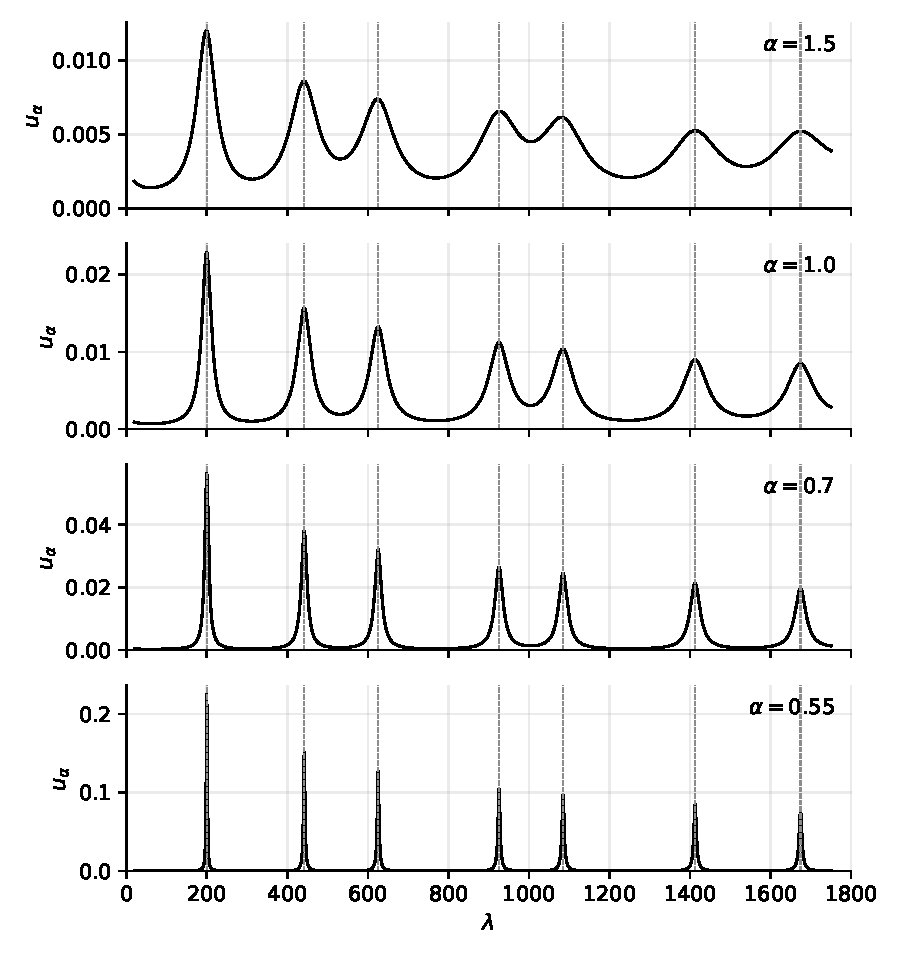
\includegraphics[width=\textwidth]{fig/maxwald_basepoint.pdf}
\caption{The density $u_\alpha$ of \eqref{eq:Ualpha}, computed from $\re\,\xi'/\xi$ on the line $\re s=\alpha$ with no zero as input, for $\alpha=1.5,1,0.7,0.55$; for $\alpha=0.7$ and $0.55$ it is the Thorin density of $T_\alpha$ only if no zero lies to the right of the line, as under RH. Dashed lines mark $\gamma_k^2$. The term of a zero on the line has unit mass and is close to a Lorentzian of width $4(\alpha-\frac12)\gamma_k$ near its peak (Proposition~\ref{mw:prop:lambda}); as $\alpha\downarrow\frac12$ these terms converge to unit atoms at $\gamma_k^2$.}
\label{mw:fig:basepoint}
\end{figure}

\section{The maximum representation does not transfer}\label{mw:sec:nomax}

The distribution function of $T$ can be computed by residues, as $\vartheta_4$ is for $M_4$ (Section~\ref{sec:ch16:max}). Along a vertical line $\re\lambda=-L$ that contains no pole of $1/G$, the point $\frac12+\sqrt\lambda$ runs off to the right as $|\im\lambda|\to\infty$, where $|\xi|$ grows, so $1/(\lambda G(\lambda))$ is integrable on the line and the Bromwich contour for $F_T(t)=\Pr(T\le t)$, whose transform is $1/(\lambda G(\lambda))$, can be shifted from $\re\lambda>0$ to $\re\lambda=-L$ past the finitely many poles in between, because $\re(-a_k)\le\frac14-\gamma_k^2$. Write $R_k$ for the residue of $1/G$ at $-a_k$, which for a simple zero $\rho_k=\frac12+i\gamma_k$ is $R_k=-2\gamma_k\Xi(0)/\Xi'(\gamma_k)$ (Section~\ref{sec:ch18:law}). When the poles with $\re a_k<L$ are simple,
\begin{equation}\label{mw:eq:survival}
\Pr(T>t)=\sum_{\re a_k<L}\frac{R_k}{a_k}\,e^{-a_kt}+O(e^{-Lt}),\qquad t\to\infty .
\end{equation}
Only this finite shift is used below: the full residue series needs contours between the poles on which $1/|\xi|$ is controlled, and under RH with simple zeros it is the spectral expansion of Section~\ref{sec:ch18:law}.

The coefficients $R_k/a_k$ alternate in sign, because $\Xi'$ changes sign at consecutive simple zeros, and they grow like $e^{\pi\gamma_k/4}$ up to a power of $\gamma_k$ and the factor $1/|\zeta'(\rho_k)|$ (Section~\ref{sec:ch18:law}). The factor $e^{-\gamma_k^2t}$ still wins for every $t>0$.

A law $F$ on $(0,\infty)$ that is the distribution function of a maximum of independent exponential variables $E_i/r_i$ with deterministic rates $r_i$, where $\sum_ie^{-r_it}<\infty$ for $t>0$, has $-\log F(t)=\sum_i\sum_{m\ge1}e^{-mr_it}/m$, a sum of exponentials with positive coefficients. The same holds, with $-\log F(t)=\int e^{-xt}\,\nu(dx)$, for the maximum of a Poisson cloud of exponential clocks with a rate measure $\nu$, that is, of the clocks $E_i/x_i$ attached to the points $x_i$ of a Poisson process of intensity $\nu$, since the number of clocks above $t$ is Poisson with mean $\int e^{-xt}\nu(dx)$.

\begin{proposition}\label{mw:prop:nomax}
$-\log F_T$ is not completely monotone. Hence $T$ is not distributed as a maximum of independent exponential variables, for any choice of rates, nor as the maximum of a Poisson cloud of exponential clocks.
\end{proposition}

\begin{proof}
Put $q_k=R_k/a_k$. For $k\le3$ the zero $\rho_k$ lies on the line, so the $a_k=-(\rho_k-\frac12)^2$ of Section~\ref{ch:clock} equals $\gamma_k^2$. The zeros with $\re a<3a_1=599.37$ are $\rho_1$ and $\rho_2$ only: $a_1=199.79$, $a_2=441.93$ and $a_3=625.54$, the zeros below height $H=3\times10^{12}$ lie on the line \cite{PT21}, and a zero above $H$ has $\re a\ge\gamma^2-\frac14>H^2-\frac14$ wherever it lies. The zeros below height $200$ are simple (Section~\ref{sec:ch6:measure}). Equation \eqref{mw:eq:survival} with $L=3a_1$ gives $\Pr(T>t)=q_1e^{-a_1t}+q_2e^{-a_2t}+O(e^{-3a_1t})$, and since $-\log(1-y)=y+\frac12y^2+O(y^3)$ and $2a_1<a_2<3a_1<a_1+a_2$,
\[
-\log F_T(t)=q_1e^{-a_1t}+\tfrac12q_1^2e^{-2a_1t}+q_2e^{-a_2t}+O(e^{-3a_1t}).
\]
Suppose that $-\log F_T(t)=\int_{[0,\infty)}e^{-xt}\nu(dx)$ for $t>0$ with $\nu\ge0$ (Bernstein's theorem). First $\nu([0,a_1))=0$: for $x_0<a_1$, $\nu([0,x_0])e^{-x_0t}\le-\log F_T(t)=O(e^{-a_1t})$. Then $e^{a_1t}(-\log F_T(t))=\nu(\{a_1\})+\int_{(a_1,\infty)}e^{-(x-a_1)t}\nu(dx)$, whose last term tends to $0$ by dominated convergence, so $\nu(\{a_1\})=q_1$, and $f_1(t)=\int_{(a_1,\infty)}e^{-xt}\nu(dx)=\frac12q_1^2e^{-2a_1t}+q_2e^{-a_2t}+O(e^{-3a_1t})$. The same two steps give $\nu((a_1,2a_1))=0$ and $\nu(\{2a_1\})=\frac12q_1^2$, and then $f_2(t)=\int_{(2a_1,\infty)}e^{-xt}\nu(dx)\ge0$ satisfies $e^{a_2t}f_2(t)\to q_2$ because $a_2<3a_1$. So $q_2\ge0$. But $R_2=-2\gamma_2\Xi(0)/\Xi'(\gamma_2)$ and $\Xi'(\gamma_2)>0$, since $\Xi$ is positive on $[0,\gamma_1)$, negative on $(\gamma_1,\gamma_2)$ and changes sign at the simple zero $\gamma_2$; so $q_2=R_2/a_2<0$, a contradiction.
\end{proof}

For $M_4$ the coefficient at $a_2=4\pi$ also has the wrong sign: $\Pr(M_4>t)=\sum_{n\ge1}2(-1)^{n+1}e^{-\pi n^2t}$ has $q_1=2$ and $q_2=-2$. But $a_2=4\pi=4a_1$ coincides with a term of the expansion in $q_1$, and the coefficient of $e^{-4\pi t}$ in $-\log\vartheta_4$ becomes $q_2+\frac14q_1^4=-2+4=2>0$. Commensurability of the exponents $\pi n^2$ rescues complete monotonicity (the Jacobi triple product writes $-\log\vartheta_4$ as a sum of exponentials with positive coefficients), while $\gamma_2^2/\gamma_1^2=2.2119$ is not an integer, so nothing rescues it for $T$.

\section{Gnedenko: the first zero as a norming constant}\label{mw:sec:gnedenko}

Gnedenko's theorem \cite{Gnedenko43} classifies the limits of normalised maxima of independent identically distributed variables, and a law with a tail $\Pr(X>t)\sim Ce^{-at}$ lies in the Gumbel domain with norming constant $1/a$ and centring $\log(Cn)/a$. The proposition reads the norming constant of $T$ as the first atom $\gamma_1^2$ of its Thorin measure, with the constant given by the first residue.

\begin{proposition}\label{mw:prop:gnedenko}
\begin{enumerate}
\item[(i)] $\Pr(M_4>t)\sim2e^{-\pi t}$, so for independent copies $M_4^{(j)}$, $j\le n$,
\[
\Pr\big(\pi\max_{j\le n}M_4^{(j)}-\log(2n)\le x\big)\to\exp(-e^{-x}).
\]
\item[(ii)] $\Pr(T>t)\sim(R_1/\gamma_1^2)\,e^{-\gamma_1^2t}$, so for independent copies $T^{(j)}$, $j\le n$, of $T$,
\begin{gather*}
\Pr\Big(\gamma_1^2\max_{j\le n}T^{(j)}-\log\frac{R_1n}{\gamma_1^2}\le x\Big)\to\exp(-e^{-x}),\\
\max_{j\le n}T^{(j)}\Big/\log n\to\frac1{\gamma_1^2}\quad\text{in probability.}
\end{gather*}
\end{enumerate}
\end{proposition}

\begin{proof}
(i) is $1-\vartheta_4(t)=2e^{-\pi t}+O(e^{-4\pi t})$. For (ii), $T$ exists by Theorem~\ref{thm:ch12:idsd}, and \eqref{mw:eq:survival} with $a_1<L<a_2$ gives $\Pr(T>t)=(R_1/a_1)e^{-a_1t}+O(e^{-Lt})$, because the simple pole at $-\gamma_1^2$ is the rightmost singularity of $1/(\lambda G(\lambda))$ after $0$, every other pole having $\re\lambda\le-\gamma_2^2$. In both cases, if $\Pr(X>t)\sim Ce^{-at}$ and $y_n=(\log(Cn)+x)/a$, then $n\Pr(X>y_n)\to e^{-x}$ and $\Pr(\max_{j\le n}X^{(j)}\le y_n)=(1-\Pr(X>y_n))^n\to\exp(-e^{-x})$. The last statement follows because $a\max_{j\le n}X^{(j)}-\log n$ is then tight.
\end{proof}

This gives a way to find $\gamma_1$ that uses no zeros at all: invert the Laplace transform $(1-1/G(\lambda))/\lambda$ numerically and read off the exponential rate of the tail. It is the experiment of Section~\ref{sec:ch18:law}, where the hazard of $T$ tends to $\gamma_1^2$ by Talbot inversion with no zero as input. The local logarithmic slopes of $\Pr(T>t)$ on $[0.04,0.05]$, $[0.05,0.06]$, $[0.06,0.07]$ and $[0.07,0.08]$ are $199.496$, $199.764$, $199.788$ and $199.790$, converging to $\gamma_1^2=199.7905$ at the rate $e^{-(\gamma_2^2-\gamma_1^2)t}$ predicted by the second term of \eqref{mw:eq:survival}, and the intercept $e^{\gamma_1^2t}\Pr(T>t)$ at $t=0.08$ gives $R_1/\gamma_1^2=50.87103$ against the residue value $50.87104$.

\section{Finding the zeros from the Thorin density in the \texorpdfstring{$z$}{z} chart}\label{mw:sec:zeros}

Theorem~\ref{mw:thm:stieltjes} gives a procedure in the chart $z=\lambda$: compute the smoothed Thorin density $r_\eta$ of that theorem on a grid from $\xi'/\xi$, with no zero used, locate its local maxima, and take square roots. Under RH $r_\eta=P_\eta*U_{\RH}$ is the Poisson smoothing of the Thorin measure $U_{\RH}=\sum_k\delta_{\gamma_k^2}$ at distance $\eta$ below the cut (Theorem~\ref{mw:thm:stieltjes} and Section~\ref{ch:ggc}), so each atom appears as a spike of unit mass and height near $1/(\pi\eta)$ at $x\approx\gamma_k^2$. The book carries out the same recovery in the chart $\theta=\sqrt z$ (Sections~\ref{sec:ch6:measure} and \ref{ch:deconv}). The table below is a cross check in the other chart, at $\eta=3$.

\begin{figure}[htbp]
\centering
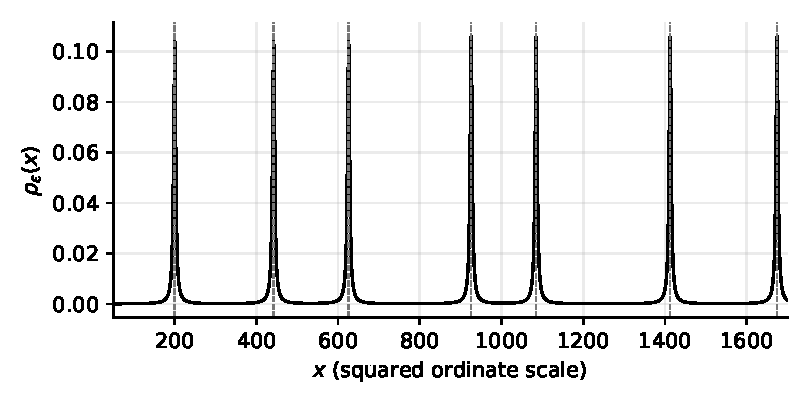
\includegraphics[width=0.8\textwidth]{fig/maxwald_thorin.pdf}
\caption{The smoothed Thorin density $r_\eta$ of $T$, $\eta=3$, computed from $\xi'/\xi$ with no zero as input. Dashed lines mark $\gamma_k^2$. Each spike has height near $1/(\pi\eta)$ and unit mass.}
\label{mw:fig:thorin}
\end{figure}

\begin{table}[htbp]
\centering\small
\begin{tabular}{rrrr}
\toprule
$k$ & peak of $r_\eta$ & $\sqrt{\text{peak}}$ & $\gamma_k$ \\
\midrule
1 & 199.790462 & 14.1347254 & 14.1347251 \\
2 & 441.926159 & 21.0220398 & 21.0220396 \\
3 & 625.542987 & 25.0108574 & 25.0108576 \\
4 & 925.673105 & 30.4248764 & 30.4248761 \\
5 & 1084.718263 & 32.9350613 & 32.9350616 \\
6 & 1412.720791 & 37.5861782 & 37.5861782 \\
7 & 1674.341571 & 40.9187191 & 40.9187190 \\
\bottomrule
\end{tabular}
\caption{Zeros recovered as atoms of the smoothed Thorin measure, $\eta=3$. The integral of $r_\eta$ over $[50,1700]$ is $6.95$, against $7$ zeros.}
\label{mw:tab:zeros}
\end{table}

The peak of $r_\eta$ near $\gamma_k^2$ is displaced from it by the pull of the neighbouring spikes, to leading order by $\eta^4\sum_{j\ne k}(\gamma_j^2-\gamma_k^2)^{-3}$, which is of modulus below $2\times10^{-5}$ in the table. On the window $[50,1700]$ with $\eta=3$ the minimum of $r_\eta$ is $5.6\times10^{-5}>0$, attained at the endpoint $x=50$. This is a consistency check of the computation with Theorem~\ref{mw:thm:stieltjes}(d) and Lemma~\ref{mw:lem:detect}, not a test of RH: the window contains only the squares of the zeros below height $\sqrt{1700}=41.2$, which are known to lie on the line.
